\documentclass[tikz,crop]{standalone}
\usetikzlibrary{automata,arrows}

\begin{document}
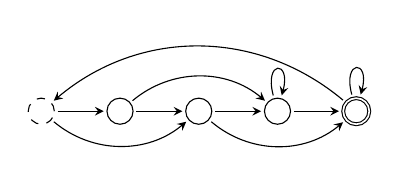
\begin{tikzpicture}
  [bend angle=40,every node/.style={draw,circle}]

  \tikzstyle{initial} = [dashed]

  \node[initial]   (1) at (1,0) {};
  \node            (2) at (2,0) {};
  \node            (3) at (3,0) {};
  \node            (4) at (4,0) {};
  \node[accepting] (5) at (5,0) {};

  \path[->, >=stealth, shorten > = 1pt, shorten < = 1pt]
        (1) edge              (2)
        (1) edge [bend right] (3)
        (2) edge              (3)
        (2) edge [bend left]  (4)
        (3) edge              (4)
        (3) edge [bend right] (5)
        (4) edge              (5)
        (4) edge [loop above] (4)
        (5) edge [loop above] (5)
        (5) edge [bend right] (1);
\end{tikzpicture}
\end{document}
%%% Local Variables:
%%% mode: latex
%%% TeX-master: t
%%% End:
